% ============================================================
%  TASK 3.2 — ONE-DIODE TOPOLOGY WITH MICROSTRIP LINES
%  RF Energy Harvesting Report
% ============================================================

\section{Task 3.2 --- One-Diode Topology with Microstrip Lines}
\label{sec:task3_2}

This section repeats steps~(4) and~(5) from Task~3.1, progressively
replacing the components of the matching network with microstrip
lines.
The goal is to move closer to a circuit that can realistically be
implemented on a PCB, where the physical traces play an active role in
impedance matching, and to compare the results with those obtained using
only LC circuit.

% ------------------------------------------------------------
\subsection{Substrate and design rules}
\label{subsec:design_rules}
% ------------------------------------------------------------

The physical PCB implementation has specific design rules for this
project :
%
\begin{itemize}
    \item Substrate: Rogers 4350B ($\varepsilon_r = 4.5$,
          $\tan\delta = 0.02$, $H = \SI{1.6}{\milli\meter}$,
          copper thickness $T = \SI{0}{\milli\meter}$ in ADS model);
    \item Signal traces: characteristic impedance $Z_0 = \SI{50}{\ohm}$,
          corresponding to $W = \SI{3.034}{\milli\meter}$;
    \item Microstrip line length constraints:
          $\SI{3}{\milli\meter} \leq L_\mathrm{line} \leq \SI{10}{\milli\meter}$;
    \item SMD package: 0603.
\end{itemize}
%
Each lumped component (capacitor, inductor) is surrounded by two
microstrip lines on either side, connected with T-junction
elements to model the physical routing on the PCB.
All line segments use $W = \SI{3.034}{\milli\meter}$, consistent with
$Z_0 = \SI{50}{\ohm}$. Here is the global schematic : 

\begin{figure}[H]
    \centering
    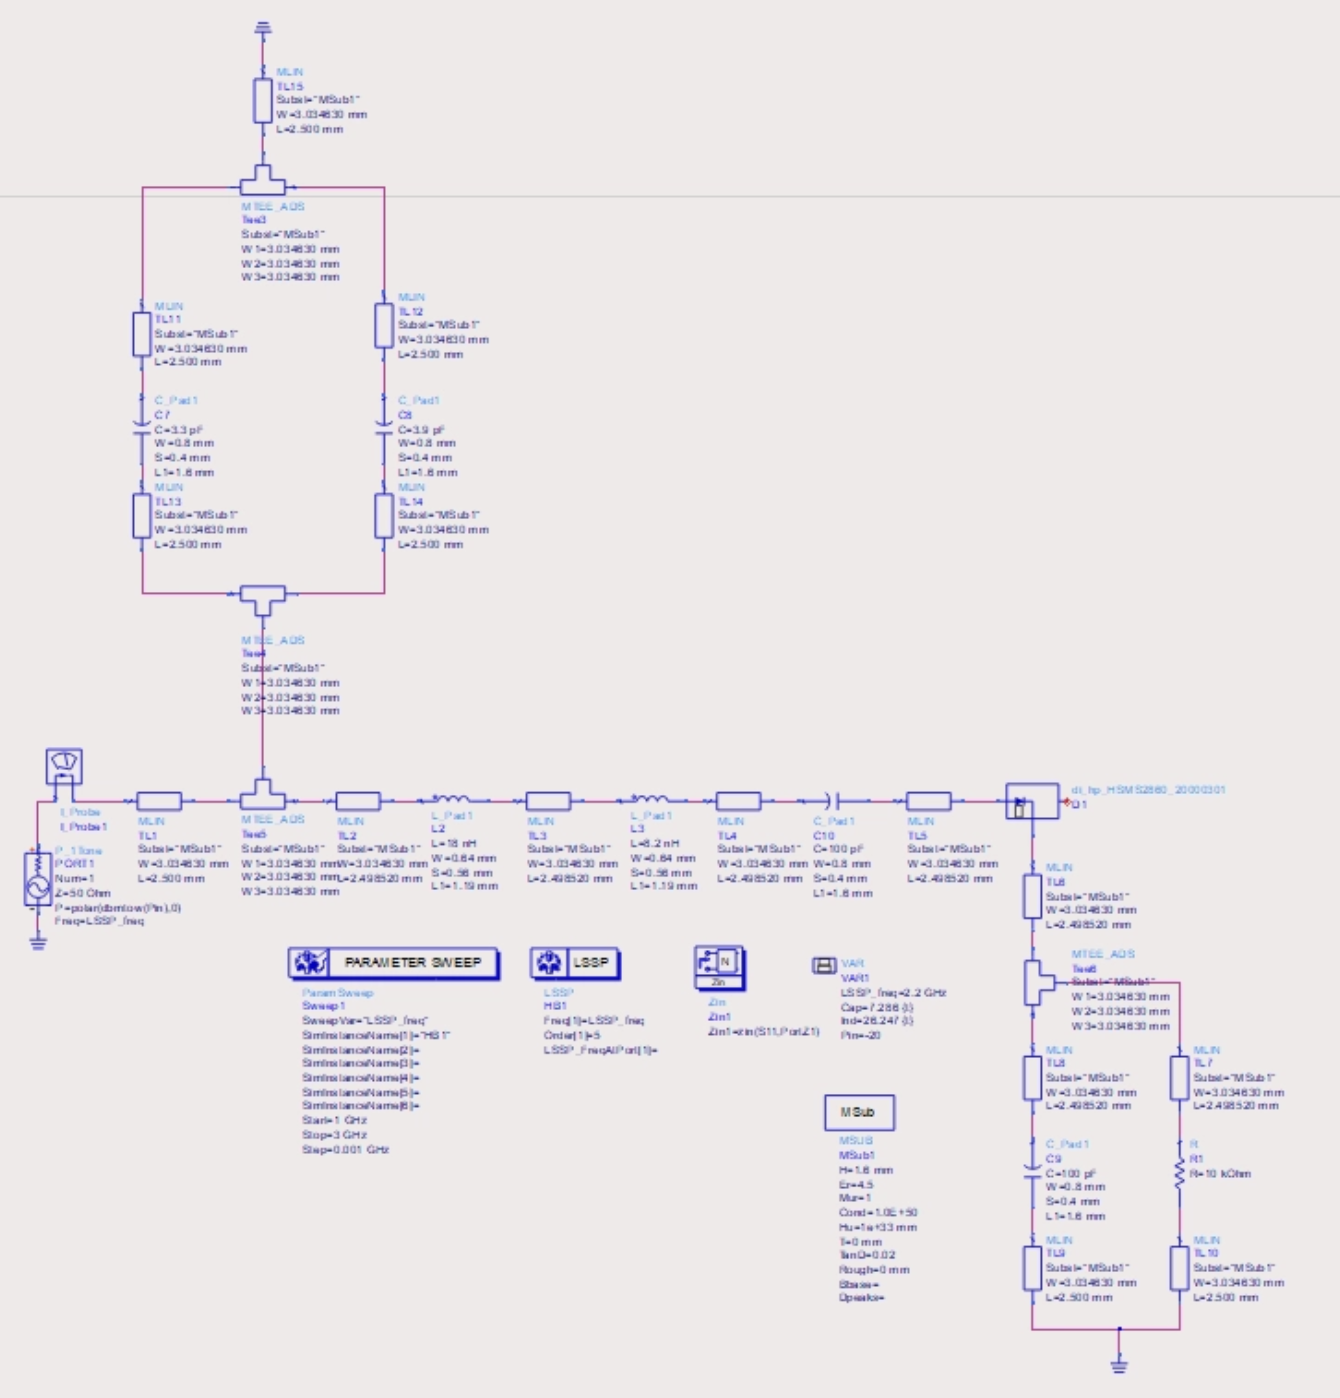
\includegraphics[width=\linewidth]{images/schema_1d_lc_ms.png}
    \caption{ADS simulation of the one-diode series rectifier, lumped-circuit and microstrip lines matching circuit.}
    \label{fig:schema_1d_lc_ms}
\end{figure}

% ------------------------------------------------------------
\subsection{Effect of microstrip parasitics on resonance frequency}
\label{subsec:mlin_parasitics}
% ------------------------------------------------------------

When the microstrip lines are introduced into the simulation while keeping
the original lumped component values unchanged, the $S_{11}$ resonance shifts from
\SI{2.2}{\giga\hertz} to approximately \SI{1.8}{\giga\hertz}
(Figure~\ref{fig:schema_1d_lc_ms}).
The degradation is caused by the additional inductance and capacitance
created by the microstrip lines, which effectively increase the total
reactive energy stored in the network.
A re-tuning of the matching circuit is therefore required to restore the
resonance at the target frequency.

\begin{figure}[H]
    \centering
    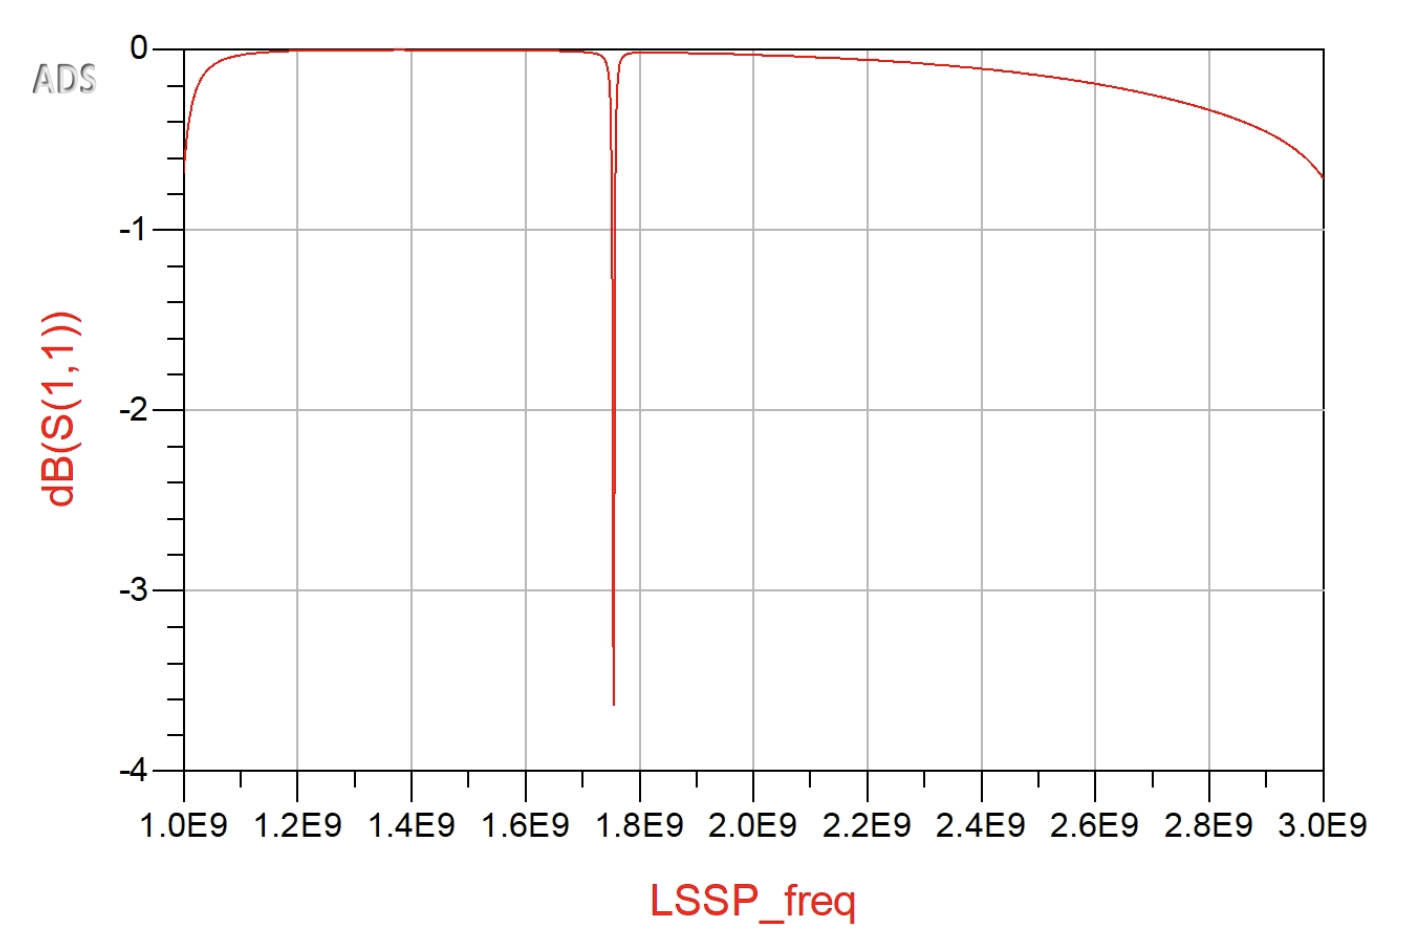
\includegraphics[width=\linewidth]{images/result_1d_S11_decale.png}
    \caption{$S_{11}$ of the lumped matching circuit with microstrip
             lines, before re-tuning.}
    \label{fig:result_1d_S11_decale}
\end{figure}

After re-tuning microstip lengths (L), capacitors (Cap) and inductors (Ind) values, we obtained these values and results : 

\begin{figure}[H]
    \centering
    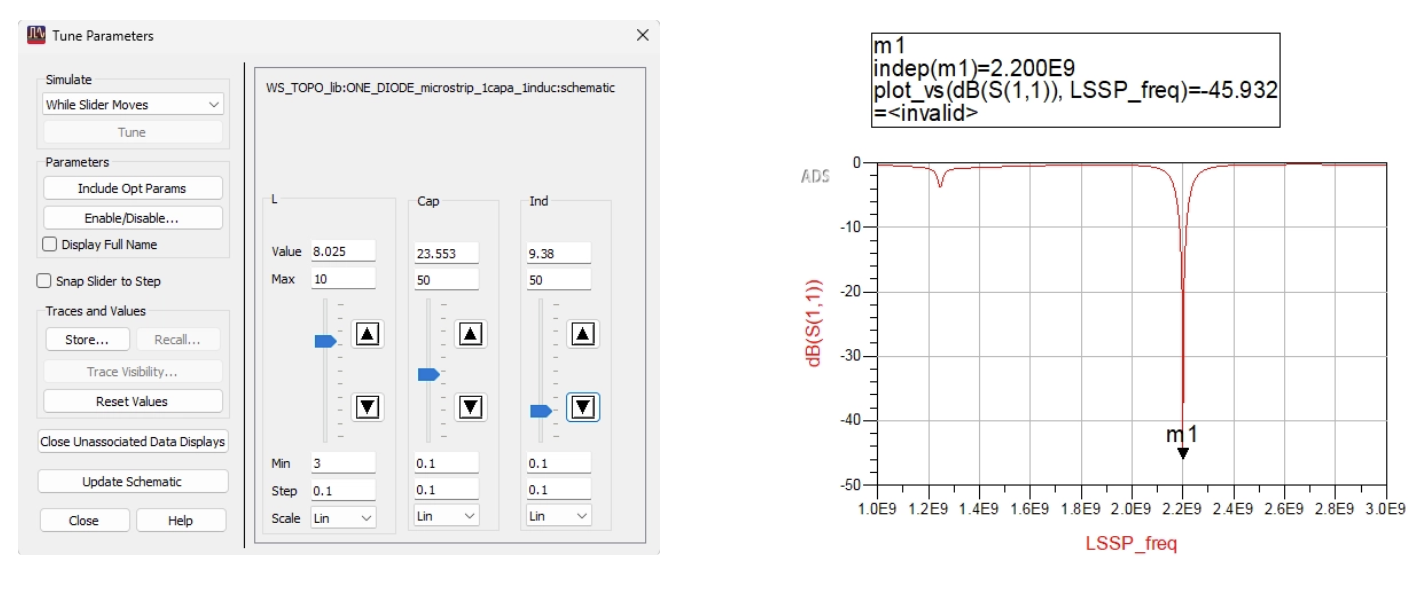
\includegraphics[width=0.75\linewidth]{images/result_1d_S11_param_lcl.png}
    \caption{$S_{11}$ of the lumped matching circuit with microstrip
            lines, after re-tuning \& parameters values.}
    \label{fig:result_1d_S11_param_lcl}
\end{figure}

By tuning our different parameters, we found right values : 
\begin{equation}
    L = \SI{8.025}{\milli\meter}, \quad
    C = \SI{23.553}{\pico\farad}, \quad
    L_\mathrm{ind} = \SI{9.38}{\nano\henry}.
\end{equation}

With those, we obtain a $S_{11}$ way below $-10$\,dB at our frequency of $2.2\,\mathrm{GHz}$ which is following specifications. 

% ------------------------------------------------------------
\subsection{Simplified 1C-1L topology with re-tuning}
\label{subsec:simplified_1c1l}
% ------------------------------------------------------------

To reduce design complexity and component count, the two-stage LC circuit is
simplified to a single capacitor and a single inductor. Here is the new schematic : 

\begin{figure}[H]
    \centering
    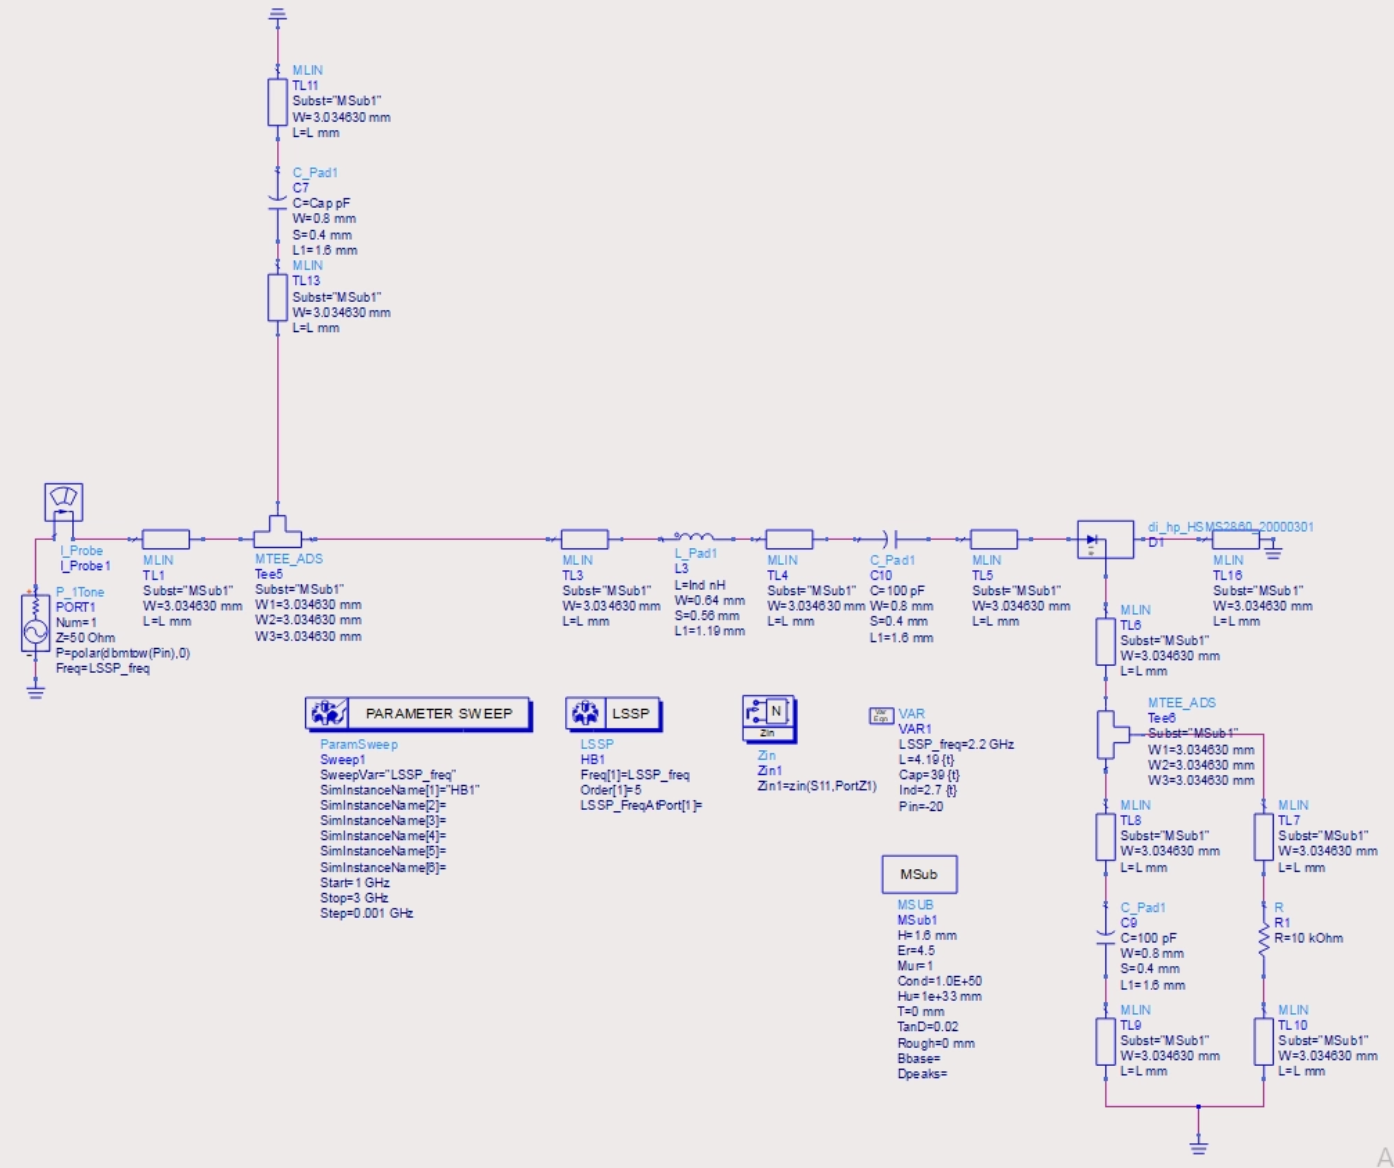
\includegraphics[width=\linewidth]{images/schema_1d_lc_ms_simple.png}
    \caption{ADS simulation of the one-diode series rectifier, lumped-circuit and microstrip lines matching circuit simplified.}
    \label{fig:schema_1d_lc_ms_simple}
\end{figure}

A parameter sweep in ADS over the line length $L$, the capacitance
$\mathrm{Cap}$, and the inductance $\mathrm{Ind}$ determined the following values:
%
\begin{equation}
    L = \SI{4.19}{\milli\meter}, \quad
    C = \SI{39}{\pico\farad}, \quad
    L_\mathrm{ind} = \SI{2.7}{\nano\henry}.
    \label{eq:opt_1c1l}
\end{equation}
%
With these values, the $S_{11}$ at \SI{2.2}{\giga\hertz} achieves:
%
\begin{align}
    S_{11} &= \SI{-31.37}{\deci\bel}
        \quad (\text{marker m1}), \\
    S_{11}&= \SI{-15.41}{\deci\bel}
        \quad (\text{marker m2}).
\end{align}
%
The results are shown in Figure~\ref{fig:s11_1c1l_retuned} :
\begin{figure}[H]
    \centering
    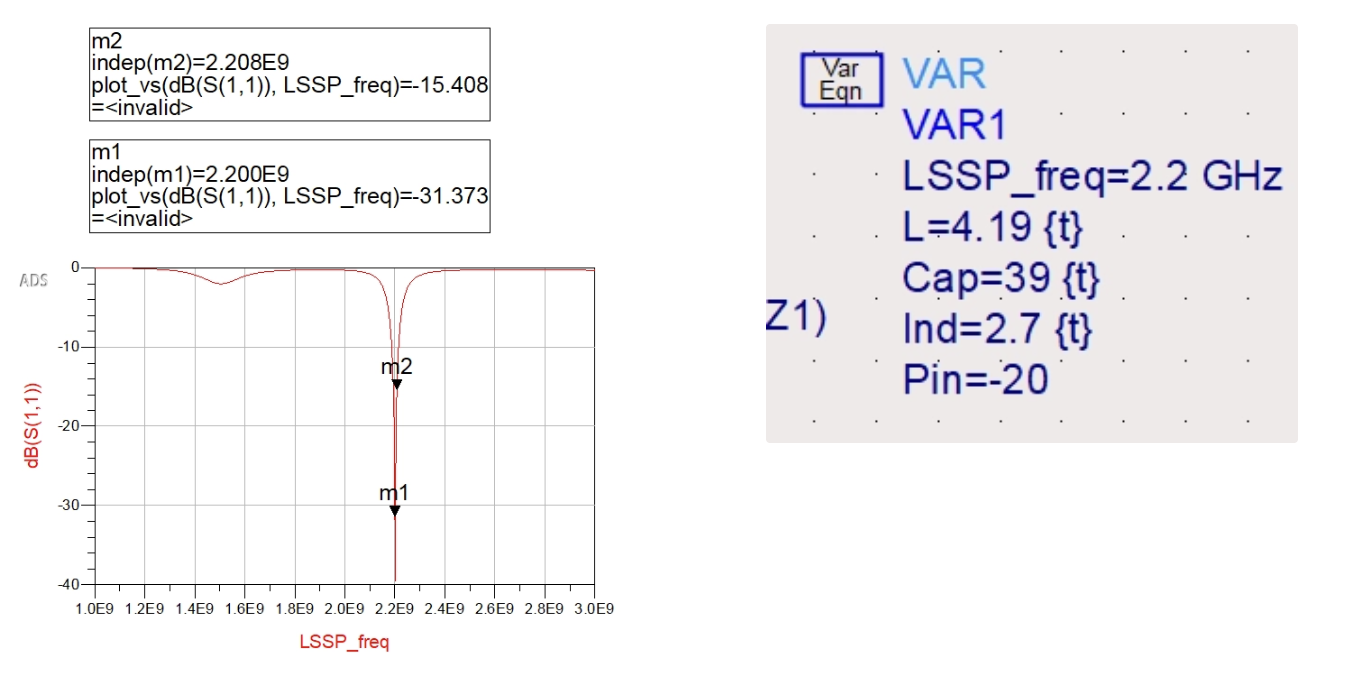
\includegraphics[width=\linewidth]{images/s11_1c1l_retuned.png}
    \caption{$S_{11}$ of the simplified 1C--1L matching circuit with
             microstrip segments, after parameter sweep re-tuning.}
    \label{fig:s11_1c1l_retuned}
\end{figure}

The specification $S_{11} < \SI{-10}{\deci\bel}$ is satisfied at \SI{2.2}{\giga\hertz},
confirming that the simplified topology is well adapted after re-tuning.

% ------------------------------------------------------------
\subsection{Fully distributed microstrip implementation}
\label{subsec:full_ms}
% ------------------------------------------------------------

For the final step, the capacitor and inductor are replaced by
microstrip lines acting as inductor and capacitor elements.
This topology eliminates the dependency on SMD components.

Here is the global schematic of this implementation : 
\begin{figure}[H]
    \centering
    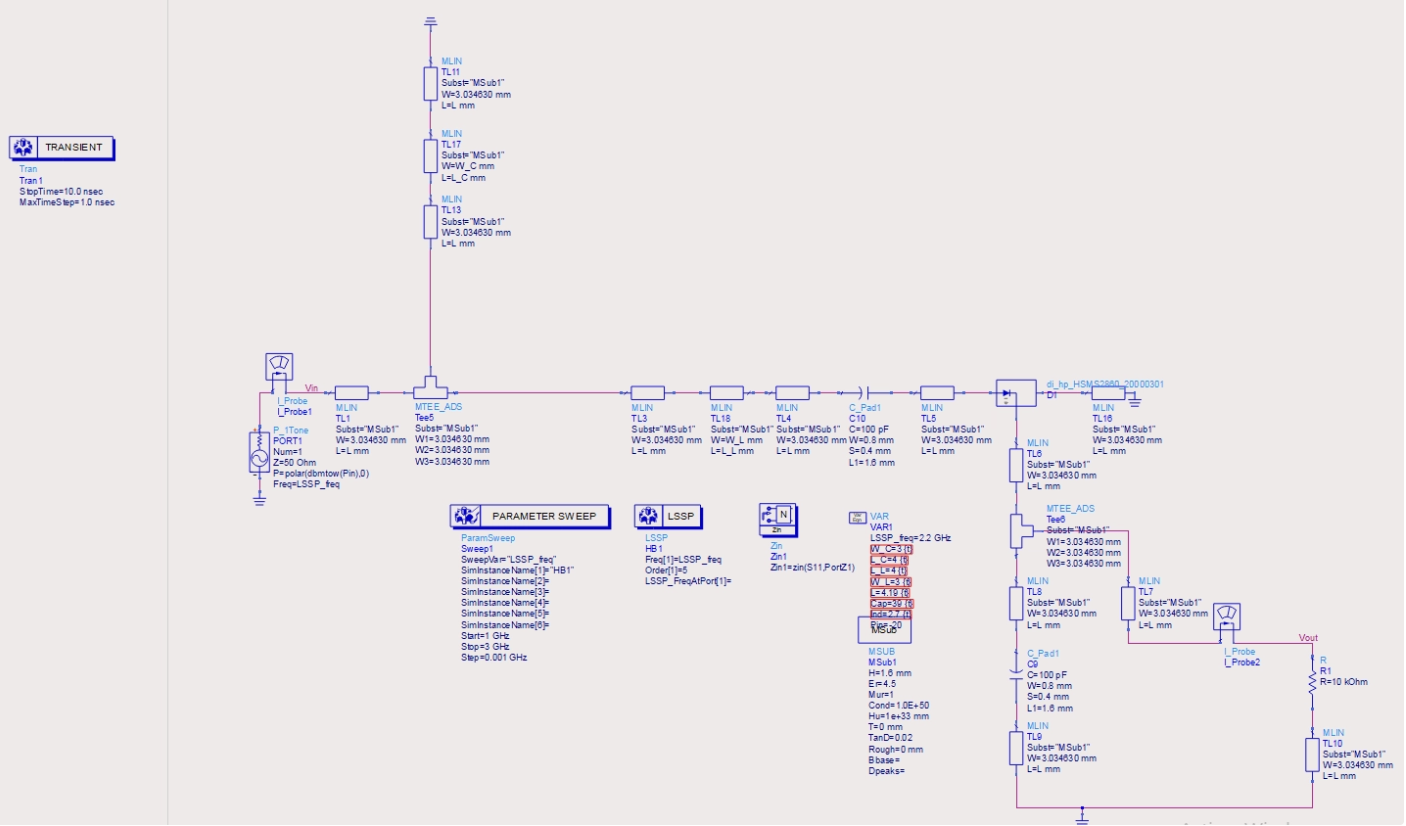
\includegraphics[width=\linewidth]{images/schema_1d_onlymc.png}
    \caption{ADS simulation of the one-diode series rectifier with only microstrip lines matching circuit.}
    \label{fig:schema_1d_onlymc}
\end{figure}

For this new implementation, new tuning have been also done for sure. Here is the result and correct parameters values : 

\begin{figure}[H]
    \centering
    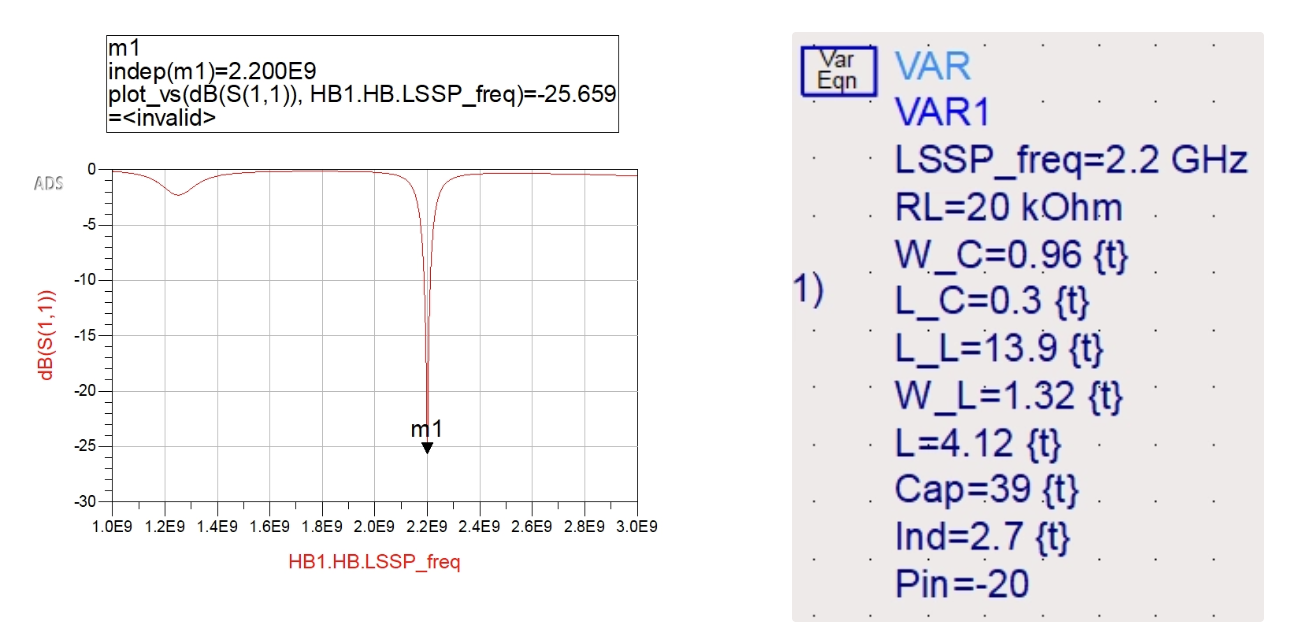
\includegraphics[width=\linewidth]{images/result_1d_onlymc.png}
    \caption{$S_{11}$ of the only microstrip lines matching circuit, after parameter sweep re-tuning.}
    \label{fig:result_1d_onlymc}
\end{figure}

The full set of tuning parameters and their optimal values after the ADS
Tune optimization are listed in Table~\ref{tab:microstrip_only_tune}.

\begin{table}[H]
    \centering
    \caption{Optimized parameter values for the full microstrip
             matching circuit (one-diode topology, \SI{2.2}{\giga\hertz}).}
    \label{tab:microstrip_only_tune}
    \begin{tabular}{lll}
        \toprule
        Parameter & Physical meaning & Optimized value \\
        \midrule
        $W_C$ & Width of capacitive stub      & \SI{0.96}{\milli\meter} \\
        $L_C$ & Length of capacitive stub     & \SI{0.3}{\milli\meter} \\
        $L_L$ & Length of inductive stub      & \SI{13.9}{\milli\meter} \\
        $W_L$ & Width of inductive stub       & \SI{1.32}{\milli\meter} \\
        $L$   & Main line segment length      & \SI{4.12}{\milli\meter} \\
        Cap   & Residual lumped capacitance   & \SI{39}{\pico\farad} \\
        Ind   & Residual lumped inductance    & \SI{2.7}{\nano\henry} \\
        \bottomrule
    \end{tabular}
\end{table}

With this fully distributed configuration, the $S_{11}$ reaches
\textbf{\SI{-25.66}{\deci\bel}} at \SI{2.2}{\giga\hertz}
(Figure~\ref{fig:result_1d_onlymc}), representing the best matching
performance achieved in this study.
The very deep and narrow resonance maximizes power transfer at our frequency at the cost of a
reduced matching bandwidth.

% ------------------------------------------------------------
\subsection{Rectifier Performance and Topology Comparison}
\label{subsec:performance_comparison}
% ------------------------------------------------------------

In this final stage, the full behavior of the one-diode topology is evaluated. We compare the ideal lumped LC matching circuit (designed in Task~3.1) with the physical microstrip circuit (designed in Task~3.2) across two main criteria: impedance matching ($S_{11}$) and RF-to-DC power conversion efficiency ($\eta$).

\subsubsection{Impedance Matching ($S_{11}$) Comparison}

Figure~\ref{fig:s11_comparison_t32} overlays the $S_{11}$ curves for the two configurations:
%
\begin{itemize}
    \item \textbf{Lumped LC circuit}: ideal SMD components, without modeling of the PCB traces;
    \item \textbf{Microstrip circuit}: capacitor and inductor replaced by physical \texttt{MLIN} blocks.
\end{itemize}

\begin{figure}[H]
    \centering
    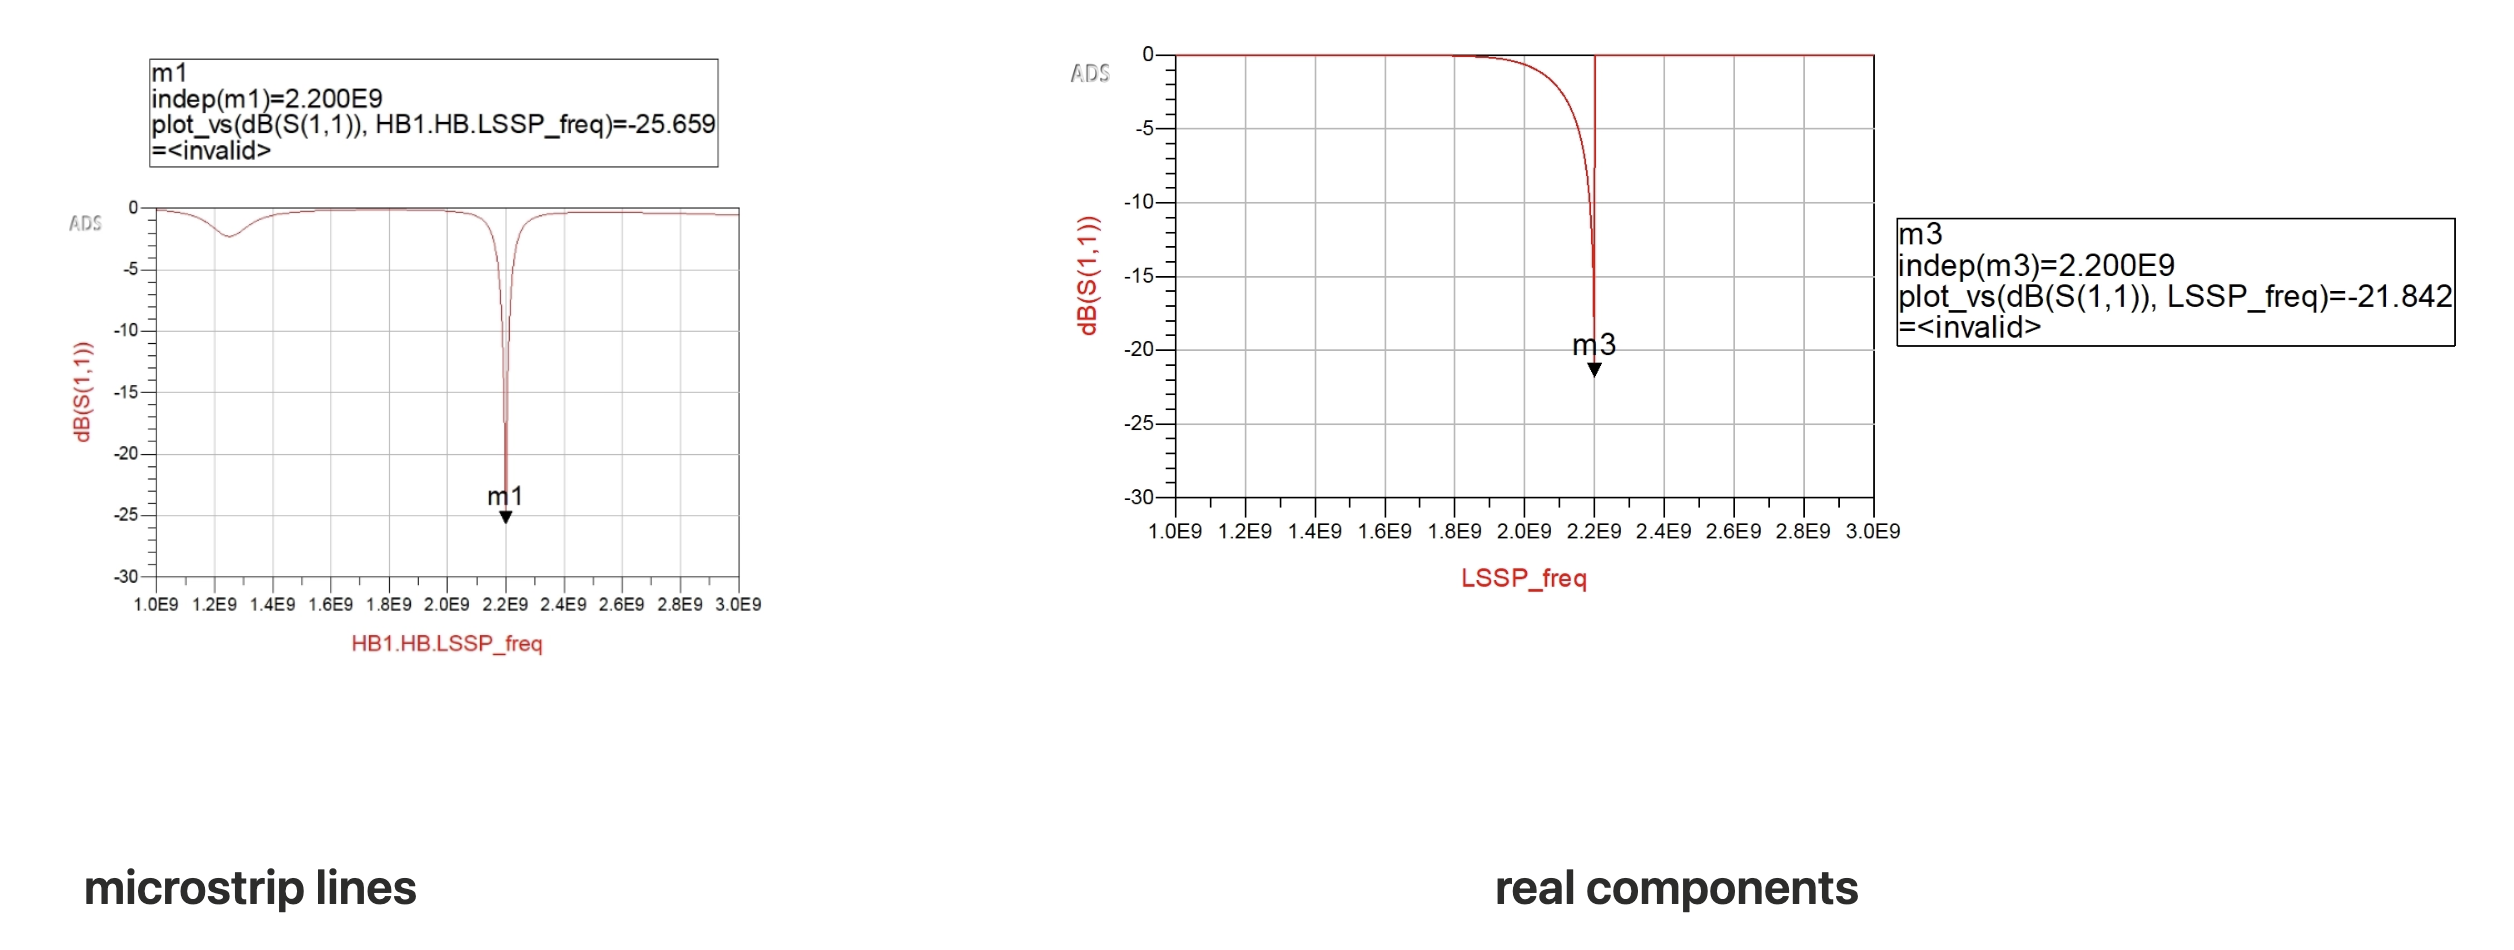
\includegraphics[width=0.75\linewidth]{images/s11_comparison_t32.png}
    \caption{Comparison of $S_{11}$ between the lumped LC matching circuit (Task~3.1) and the microstrip circuit (Task~3.2). $R_L = \SI{20}{\kilo\ohm}$, $P_\mathrm{in} = -20$\,dBm.}
    \label{fig:s11_comparison_t32}
\end{figure}

\paragraph{Impedance Matching Analysis}
Both circuits achieve to reach the right impedance matching at \SI{2.2}{\giga\hertz} ($S_{11} < \SI{-15}{\deci\bel}$), but their behaviors are quite different. The microstrip topology achieves a deeper $S_{11}$ dip, since the line dimensions allow continuous tuning, unlike the discrete values of L\&C components.
\subsubsection{Power Conversion Efficiency (\texorpdfstring{$\eta$}{eta}) and DC Output}

The RF-to-DC power conversion efficiency (PCE) is defined as the ratio of the rectified DC power delivered to the load over the incident RF power:
%
\begin{equation}
    \eta = \frac{P_\mathrm{DC}}{P_\mathrm{RF}}
         = \frac{V_\mathrm{out} \cdot I_\mathrm{out}}{V_\mathrm{in} \cdot I_\mathrm{in}}
         \times 100\,\%.
    \label{eq:pce}
\end{equation}

To accurately evaluate the performance of our system, a Large-Signal Harmonic Balance (HB) simulation was performed. The load resistance was adjusted to $R_L = \SI{20}{\kilo\ohm}$ to precisely model the equivalent input resistance of the chosen STTS22H sensor.

\paragraph{Performance of the Lumped LC Matching Circuit}
First, we simulated the topology using ideal SMD components for the matching network. Figure~\ref{fig:perf_lc_6graphs} presents the full set of results (Efficiency and Output Voltage as functions of both Input Power and Load Resistance).

\begin{figure}[H]
    \centering
    %\includegraphics[width=\linewidth]{images/perf_lc.png} % <-- Mets ici ta capture des 6 graphiques de la page 32
    \caption{Performance dashboard (Efficiency $\eta$ and $V_\mathrm{out}$) for the 1-Diode topology with Lumped LC matching ($f = \SI{2.2}{\giga\hertz}$, $R_L = \SI{20}{\kilo\ohm}$).}
    \label{fig:perf_lc_6graphs}
\end{figure}

At our maximum targeted input power ($P_\mathrm{in} = \SI{10}{\dBm}$), the efficiency reaches approximately \textbf{6.69\%}.

\paragraph{ Performance of the Full Microstrip Circuit}
Next, we evaluated the final physical implementation where the matching network relies solely on microstrip lines. The results are shown in Figure~\ref{fig:perf_ms_6graphs}.

\begin{figure}[H]
    \centering
    %\includegraphics[width=\linewidth]{images/perf_ms.png} % <-- Mets ici ta capture des 6 graphiques de la page 33
    \caption{Performance dashboard (Efficiency $\eta$ and $V_\mathrm{out}$) for the 1-Diode topology with fully distributed Microstrip matching ($f = \SI{2.2}{\giga\hertz}$, $R_L = \SI{20}{\kilo\ohm}$).}
    \label{fig:perf_ms_6graphs}
\end{figure}

With the microstrip matching network, the efficiency at $P_\mathrm{in} = \SI{10}{\dBm}$ improves drastically, reaching \textbf{17.15\%}. 

\paragraph{Efficiency Analysis}
This significant improvement (from 6.69\% to 17.15\%) can be explained by the physical nature of the matching networks. Ideal lumped inductors and capacitors have inherent parasitic series resistances ($R_s$) that dissipate RF energy as heat. By replacing them with fully distributed microstrip lines on a high-quality RF substrate (Rogers 4350B), we reduce these insertion losses, leading to a higher quality factor (Q) and better energy transfer to the diode.

\subsubsection{Adequacy for powering the STTS22H sensor}

The ultimate goal of this rectifier is to power an STTS22H temperature sensor. According to its datasheet, the sensor requires a supply voltage between \SI{1.5}{\volt} and \SI{3.6}{\volt}, and consumes a maximum active current of \SI{120}{\micro\ampere}. 

The absolute minimum DC power required is:
%
\begin{equation}
    P_\mathrm{DC,min}
    = V_\mathrm{DD,min} \times I_\mathrm{DD,max}
    = \SI{1.5}{\volt} \times \SI{120}{\micro\ampere}
    = \SI{180}{\micro\watt}.
\end{equation}

Using our final microstrip implementation at an input power of $P_\mathrm{in} = \SI{10}{\dBm}$ (which equals \SI{10}{\milli\watt}), the measured efficiency is $\eta = 17.15\%$. 
The delivered DC power is therefore:
\begin{equation}
    P_\mathrm{DC,delivered} = \SI{10}{\milli\watt} \times 0.1715 = \SI{1.715}{\milli\watt} = \SI{1715}{\micro\watt}.
\end{equation}

\paragraph{Conclusion}
The delivered power (\SI{1715}{\micro\watt}) is nearly ten times higher than the strict minimum required (\SI{180}{\micro\watt}). Furthermore, the Harmonic Balance simulation (Figure~\ref{fig:perf_ms_6graphs}) shows that at $P_\mathrm{in} = \SI{10}{\dBm}$, the output voltage $V_\mathrm{out}$ reaches approximately \SI{2.5}{\volt} to \SI{3.0}{\volt}, which sits perfectly within the sensor's safe operating range (\SIrange{1.5}{3.6}{\volt}). 

We can confidently conclude that the one-diode microstrip topology is fully capable of powering the STTS22H sensor under these RF conditions.